In this section, we prove a similar result for convex hull scores:
\begin{Definition}
  Let $X$ be the sphere or the plane, and let $U\subset X$ be some 
  open region with finite area. Let $Conv(U)$ be the convex hull of 
  $U$ in $X$. We define the {\bf convex hull} score of $U$ by:
  \begin{align*}
    CH_X(U) = \frac{\text{Area}(U)}{\text{Area}(Conv(U))}
  \end{align*}
\end{Definition}
\abn{should we prove that the convex hull of a finite area shape is 
measureable and of finite area? Is this even true?}
\lsn{It's that every convex set is measurable ( https://math.stackexchange.com/questions/207609/the-measurability-of-convex-sets ) ... its not true that its always of finite area, but if the original set is bounded,then so is the convex hull}

Note that if a map $\vphi:S^2\supset U\to V\subset \R^2$ preserves 
orderings of convex hull scores, then in particular, it must preserve 
maximal elements of these scores - the convex sets. Thus, if 
$\vphi$ does not preserve convexity, then it cannot preserve orderings 
of convex hulls. For the rest of this section, we will focus on 
local diffeomorphisms which preserve convexity.
\abn{Hey, Lorenzo, what's the reference to the paper? Do we reference 
it here? maybe just the maple notebook?}
\lsn{What paper? Jeans? I think we have a more elementary proof now... we can just use the proof mentioned here: \url{https://math.stackexchange.com/questions/4458/how-do-i-map-a-spherical-triangle-to-a-plane-triangle#4505} }
...
Thus, without loss of generality, we can assume that $\vphi$ 
is the local diffeomorphism obtained by stereographically \lsn{This isn't stereographic projection; it's a Gnomic projection. If you want, you can call this a 'projection from a point', which is standard in projective geometry.} projecting the lower hemisphere of the unit sphere centered at $(0,0,-1)\in \R^3$ to 
the $xy$ plane from the center of the sphere:
\begin{center}
Placeholder picture here:
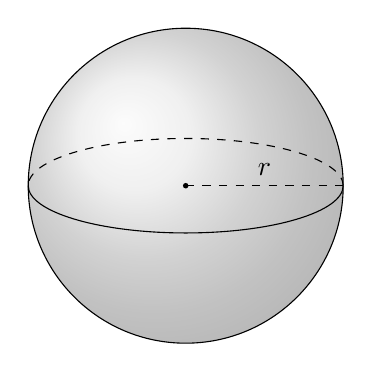
\begin{tikzpicture}
  \shade[ball color = gray!40, opacity = 0.4] (0,0) circle (2cm);
  \draw (0,0) circle (2cm);
  \draw (-2,0) arc (180:360:2 and 0.6);
  \draw[dashed] (2,0) arc (0:180:2 and 0.6);
  \fill[fill=black] (0,0) circle (1pt);
  \draw[dashed] (0,0 ) -- node[above]{$r$} (2,0);
\end{tikzpicture}
\end{center}
\begin{Definition}
Let $\theta_1<\theta_2\in \left[0, \frac{\pi}{2}\right]$ be given. Employing 
spherical co-ordinates $S^2\ni x\to (r(x),\theta(x),\phi(x))$ on $S^2$, we define:
\begin{align*}
W(\theta_1,\theta_2) 
= \{x\in S^2:\theta_1\le \phi(x)\le \theta_2\}
\end{align*}
\end{Definition}
\begin{Claim}
On $S^2$, we have:
\begin{align*}
CH(W(\theta_1,\theta_2) = \frac{\cos(\theta_1)-\cos(\theta_2)}{1-\cos(\theta_2)}
\end{align*}
and after projecting under $\vphi$, we have:
\begin{align*}
CH(\vphi(W(\theta_1,\theta_2))) 
  = 1-\frac{\tan^2(\theta_1)}{\tan^2(\theta_2)}
\end{align*}
\end{Claim}
\abn{do we need to prove this? It follows from pretty basic trigonometry}

\mute{
Here is the argument for convex hull

1. If the diffeo preserves the convex hull order, it must preserve maximal elements. These are the convex subsets. Hence it must send convex subsets to convex subsets.
2. the one dimensional convex subsets are geodesics. Hence $\phi$ must send geodesics to geodesics.
3. This means that $\phi$ must be the composition of the projection of $\psi$ with an affine trnasformation of $\mathbb{R}^2$, where $\psi$ is the projection from the center to the tangent plane through the north pole. (Gnomic projection)

Thm>
4. Now we define a washer on the sphere by $W(a,b)$. We make the following ocmputations;

1. $Area( \phi( \theta)) = \pi \tan^2(\theta)$ (area of the disc shadow)
2. $area(\theta) = 2 \pi ( 1 - cos(\theta)$ (archimedes theorem)

For $b > a$
3. $A(W(a,b)) = 2 \pi (cos (a) - cos(b))$
4. $A(conv( W(a,b)) = 2 \pi ( 1 - cos(b)$.
5. $A( \phi( W(a,b)) = \pi ( \tan^2(b) - \tan^2(a))$
6. $A( Conv( \phi( W(a,b)) = \pi \tan^2(b)$

7. Now we plug into python note book to find a,b,a',b' that flip the orders!
}